\section{Use Case Analysis}
Ziel: Abbildung der Realität in Anwendungsfalldiagramm. Dabei wird in der Regel ein konkretes Szenario beschrieben.
\begin{itemize}
	\item Use Case = Menge von Aktionssequenzen, die ein Nutzer oder externes System ausführt um ein bestimmtes Ziel zu erreichen. Beschreibt inhaltlich was beim Versuch der Zielerreichung passieren und schiefgehen kann.
	\item Helfen in der \textbf{Planungsphase}:\\
	- verdeutlichen wichtige Ziele des Produkts
	\item in der \textbf{Entwicklungsphase}\\
	- fassen Kernpunkte eines Features für Entwickler gut zusammen
	\item Erfassen der funktionalen R aus Sicht des Nutzers
\end{itemize}

\textbf{Actor:}
\begin{itemize}
	\item interagiert mit dem System; entweder Person oder wieder ein System
	\item gibt Input und erhält Output vom System
	\item extern; keine Kontrolle über den Use Case
	\item Vererbung möglich
	\item \textbf{Primär} und \textbf{Sekundär} Actor\\
	- Primär: will ein Ziel mithilfe des Systems erreichen\\
	- Sekundär: wird vom System benötigt um das Ziel des Primären zu erreichen
\end{itemize}

\begin{figure}[!h]
	\centering
	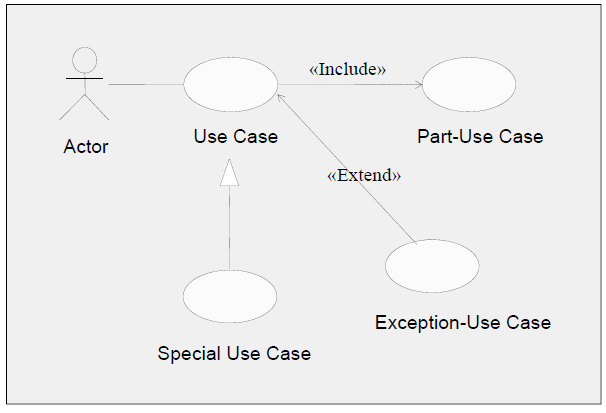
\includegraphics[scale=0.6]{img/elements_of_use_case.png}
\end{figure}